\section{Planning results}\label{sec:planresults}

\Cref{fig:planmap} shows a typical day-ahead plan.
Most trucks run on short, next-day-feasible lanes out of the large Madrid, Barcelona and Seville sites; local lanes, from an FC to the sort centre of its own city, are hidden under the markers.
The service map reveals the structural weakness of the network.
Galicia and especially northern Portugal can be reached overnight only from the small Asturias site, so a large part of their demand is delivered on day two.
We come back to this in \cref{sec:network}.

\begin{figure}[t]
  \centering
  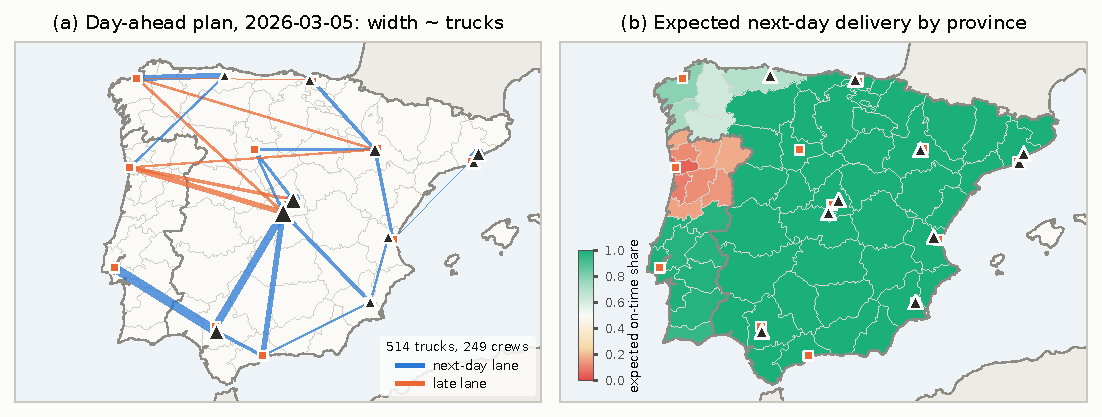
\includegraphics[width=\linewidth]{plan_map}
  \caption{(a) Day-ahead SP plan for 5 March 2026 with LightGBM+copula scenarios: line width is proportional to the number of scheduled trucks per lane (blue: next-day lane; orange: late lane); FC marker size is proportional to the scheduled crews. (b) Expected share of next-day deliveries per province under this plan, over 300 true demand scenarios.}
  \label{fig:planmap}
\end{figure}

\subsection{Statistical quality of the SAA solutions}\label{sec:saa}

How many scenarios are enough?
For a regular day (5 March 2026) and for Black Friday 2025 we solve $M=10$ independent SAA replications for each $N\in\{10,25,50,100,200,400\}$, with scenarios from the true distribution.
Every resulting plan is evaluated on the same 5000 fresh scenarios.
Following \citet{mak1999}:
\begin{itemize}
  \item the mean of the $M$ SAA optimal values is a statistical \emph{lower} bound on the true optimum (in expectation), with a $t$-based confidence interval;
  \item the best out-of-sample value is an \emph{upper} bound.
\end{itemize}

\begin{table}[t]
\centering\small
\caption{SAA bounds ($M=10$ replications per $N$, out-of-sample evaluation on 5000 true scenarios). Gap CI: 95\% upper confidence bound on the optimality gap of the best plan, $(\mathrm{UB}-\mathrm{LB}+\mathrm{hw})/\mathrm{UB}$. Time: mean Benders solve time (24 workers).}\label{tab:saa}
\resizebox{\linewidth}{!}{\begin{tabular}{@{}lrrrrrrr@{}}\toprule
Day & $N$ & Lower bound (95\% CI) & Best UB & Mean UB & Gap (\%) & Gap CI (\%) & Time (s) \\ \midrule
\multirow{6}{*}{2025-11-28} & 10 & 4{,}609{,}718 $\pm$ 61{,}195 & 4{,}609{,}066 & 4{,}611{,}047 & -0.014 & 1.314 & 0.5 \\
 & 25 & 4{,}608{,}203 $\pm$ 28{,}740 & 4{,}609{,}334 & 4{,}609{,}642 & 0.025 & 0.648 & 0.4 \\
 & 50 & 4{,}609{,}204 $\pm$ 15{,}447 & 4{,}608{,}596 & 4{,}609{,}259 & -0.013 & 0.322 & 0.7 \\
 & 100 & 4{,}608{,}588 $\pm$ 16{,}167 & 4{,}607{,}959 & 4{,}609{,}119 & -0.014 & 0.337 & 1.2 \\
 & 200 & 4{,}611{,}299 $\pm$ 15{,}916 & 4{,}608{,}849 & 4{,}609{,}101 & -0.053 & 0.292 & 1.9 \\
 & 400 & 4{,}604{,}010 $\pm$ 9{,}490 & 4{,}608{,}717 & 4{,}608{,}990 & 0.102 & 0.308 & 3.9 \\
\midrule
\multirow{6}{*}{2026-03-05} & 10 & 2{,}288{,}673 $\pm$ 27{,}928 & 2{,}290{,}941 & 2{,}292{,}870 & 0.099 & 1.318 & 11.8 \\
 & 25 & 2{,}288{,}738 $\pm$ 13{,}196 & 2{,}290{,}634 & 2{,}291{,}043 & 0.083 & 0.659 & 7.0 \\
 & 50 & 2{,}289{,}886 $\pm$ 6{,}882 & 2{,}290{,}485 & 2{,}290{,}697 & 0.026 & 0.327 & 14.9 \\
 & 100 & 2{,}289{,}350 $\pm$ 7{,}560 & 2{,}290{,}383 & 2{,}290{,}584 & 0.045 & 0.375 & 17.5 \\
 & 200 & 2{,}291{,}186 $\pm$ 7{,}021 & 2{,}290{,}276 & 2{,}290{,}469 & -0.040 & 0.267 & 30.2 \\
 & 400 & 2{,}288{,}141 $\pm$ 4{,}345 & 2{,}290{,}262 & 2{,}290{,}520 & 0.093 & 0.282 & 30.4 \\
\bottomrule\end{tabular}
}
\end{table}

\begin{figure}[t]
  \centering
  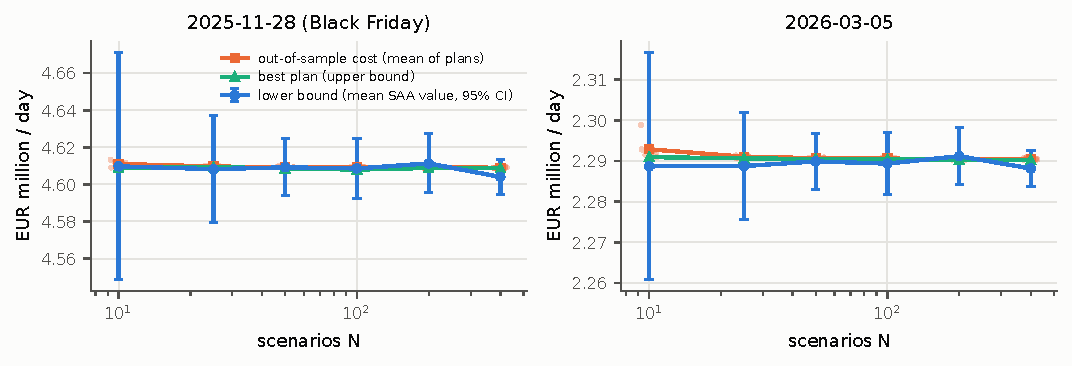
\includegraphics[width=\linewidth]{saa}
  \caption{SAA convergence. The plans' true expected cost (orange) stabilises from $N\approx 50$; the lower-bound estimator (blue, 95\% CI) tightens around it as $N$ grows.}
  \label{fig:saa}
\end{figure}

\Cref{tab:saa,fig:saa} show that the planning problem is statistically well behaved.
\begin{itemize}
  \item The true expected cost of the SAA plans stabilises quickly. Its spread across replications falls from \EUR{2239} per day at $N=10$ to about \EUR{140} at $N\ge 50$, and the plans at $N=100$ and $N=400$ differ by only \EUR{64} per day.
  \item The estimated optimality gap is statistically indistinguishable from zero for all $N\ge 25$. Its 95\% upper confidence bound falls to 0.3--0.4\% at $N\ge 50$, a level limited by the variance of the lower-bound estimator, not by the quality of the plans.
\end{itemize}
We therefore use $N=100$ throughout. Note also the optimisation tolerance of $5\cdot10^{-4}$ (\cref{sec:benders}): it is of the same order as these statistical errors, so solving more tightly would be pointless.

\paragraph{Value of the stochastic solution and of perfect information.}
\begin{table}[t]
\centering\small
\caption{Value of the stochastic solution (VSS $=$ EEV $-$ RP, paired over 5000 scenarios, $\pm$ 95\% CI) and expected value of perfect information (EVPI $=$ RP $-$ WS over 100 scenarios). RP: stochastic plan; EEV: plan for the mean demand; WS: wait-and-see.}\label{tab:vss}
\resizebox{\linewidth}{!}{\begin{tabular}{@{}lrrrrrrrr@{}}\toprule
Day & RP & EEV & VSS & WS & EVPI & Unmet \% & Trucks & Crews \\
 & \EUR{}/day & \EUR{}/day & \EUR{}/day & \EUR{}/day & \EUR{}/day & RP / EEV & RP / EEV & RP / EEV \\ \midrule
2026-03-05 & 2{,}290{,}262 & 2{,}293{,}459 & 3{,}196 $\pm$ 159 & 2{,}273{,}811 & 22{,}698 $\pm$ 2{,}602 & 0.12 / 0.03 & 519 / 530 & 252 / 257 \\
2025-11-28 & 4{,}607{,}959 & 4{,}615{,}030 & 7{,}071 $\pm$ 230 & 4{,}607{,}093 & 18{,}130 $\pm$ 1{,}590 & 0.79 / 0.77 & 954 / 952 & 425 / 425 \\
\bottomrule\end{tabular}
}
\end{table}

\Cref{tab:vss} decomposes the value of information.
\begin{itemize}
  \item \textbf{VSS.} The stochastic plan saves \EUR{3.2}k per day on the regular day and \EUR{7.1}k on Black Friday over the plan for mean demand. This is small (0.14\% and 0.15\%) but highly significant.
  \item \textbf{EVPI.} Perfect information would be worth \EUR{18}--\EUR{23}k per day, six to seven times more. Better \emph{information}, i.e.\ forecasts, matters more than better \emph{modelling of uncertainty}, consistent with \cref{sec:value-forecast}.
  \item \textbf{Direction of the hedge.} The SP plan buys \emph{fewer} trucks (519 vs.\ 530) and crews (252 vs.\ 257) than the mean-value plan. This is the newsvendor logic. Scheduled capacity costs $c$ and its same-day substitutes cost $1.6c$ (overtime) and $1.8c$ (spot), so the critical ratio $(1.8c-c)/(1.8c)\approx0.44$ is below one half. It is optimal to plan \emph{below} the mean and buy flexibility on the day. A planner who reasons only in terms of point forecasts would build the opposite safety margin. On Black Friday the labour limits bind (425 of 426 crews), so the hedge acts on trucks only.
\end{itemize}

\subsection{When does stochastic planning pay?}\label{sec:flex}\label{sec:sensitivity}

The modest VSS of the base case is a property of the cost structure, not of the method.
Same-day substitutes for scheduled capacity are only 60--80\% more expensive, and overtime can add 30\%.
We therefore vary the \emph{flexibility of recourse} on four regular days spread over the year:
\begin{itemize}
  \item the spot premium, from $1.4\times$ to $3.5\times$;
  \item the overtime cap, 30\% or 10\% of planned labour;
  \item the penalty for an unshipped unit, from \EUR{9} to \EUR{50}.
\end{itemize}
For each setting we compute the VSS and the reduction of the 95\% conditional value-at-risk (CVaR$_{95}$, the mean of the worst 5\% of days) on the true distribution.
In a second experiment (10 regular days) we repeat the forecast-based comparison of \cref{sec:value-forecast} under base and inflexible recourse.

\begin{table}[t]
\centering\small
\caption{Value of the stochastic solution as a function of recourse flexibility (means over four regular test days; SP and mean-value plans evaluated on 1000 true scenarios). $\Delta$CVaR$_{95}$: reduction of the expected cost of the worst 5\% of days achieved by the SP plan.}\label{tab:sensitivity}
\resizebox{\linewidth}{!}{\begin{tabular}{@{}rrrrrrrrrr@{}}\toprule
Spot & Overtime & Unmet & VSS & 95\% & VSS & Trucks & Crews & Unmet (\%) & $\Delta$CVaR$_{95}$ \\
premium & cap (\%) & penalty & \EUR{}/day & $\pm$ & \% & RP / EEV & RP / EEV & RP / EEV & \EUR{}/day \\ \midrule
1.4 & 10 & 15 & 4{,}382 & 199 & 0.17 & 553 / 576 & 284 / 286 & 0.09 / 0.09 & 19{,}216 \\
1.4 & 30 & 15 & 3{,}221 & 253 & 0.13 & 552 / 576 & 282 / 286 & 0.06 / 0.03 & -3{,}564 \\
1.8 & 10 & 15 & 3{,}654 & 203 & 0.15 & 569 / 578 & 284 / 286 & 0.14 / 0.12 & 19{,}666 \\
1.8 & 30 & 9 & 3{,}256 & 169 & 0.13 & 535 / 550 & 272 / 278 & 1.81 / 1.56 & 1{,}998 \\
1.8 & 30 & 15 & 2{,}552 & 164 & 0.10 & 572 / 578 & 282 / 286 & 0.10 / 0.05 & 1{,}835 \\
1.8 & 30 & 25 & 2{,}155 & 163 & 0.08 & 572 / 578 & 282 / 286 & 0.00 / 0.00 & 2{,}900 \\
1.8 & 30 & 50 & 2{,}183 & 209 & 0.08 & 571 / 578 & 282 / 286 & 0.00 / 0.00 & 5{,}257 \\
2.5 & 10 & 15 & 4{,}665 & 319 & 0.18 & 583 / 580 & 284 / 286 & 0.18 / 0.18 & 33{,}853 \\
2.5 & 30 & 15 & 3{,}435 & 161 & 0.14 & 582 / 580 & 282 / 286 & 0.15 / 0.10 & 10{,}690 \\
3.5 & 10 & 15 & 7{,}662 & 459 & 0.30 & 592 / 580 & 283 / 286 & 0.25 / 0.27 & 46{,}556 \\
3.5 & 30 & 15 & 5{,}688 & 262 & 0.23 & 592 / 580 & 282 / 286 & 0.20 / 0.19 & 25{,}113 \\
\bottomrule\end{tabular}
}
\end{table}

\begin{figure}[t]
  \centering
  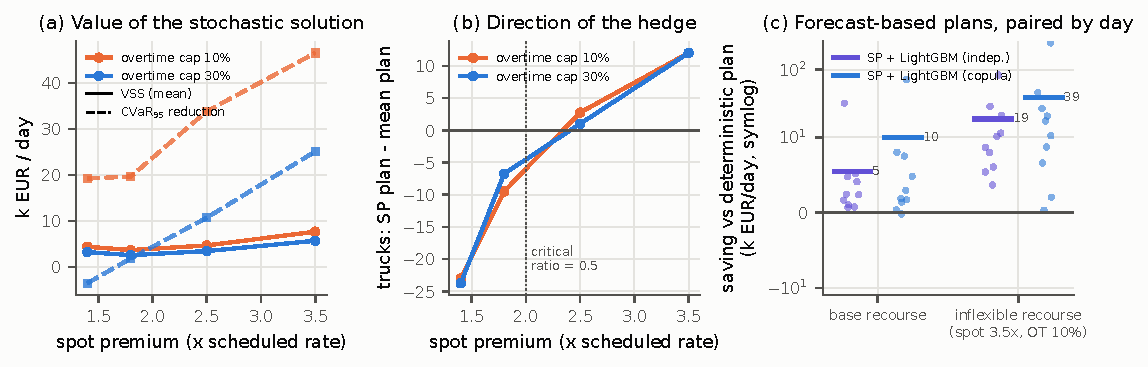
\includegraphics[width=\linewidth]{flex}
  \caption{(a) VSS (solid) and CVaR$_{95}$ reduction (dashed) against the spot premium, for two overtime caps. (b) Difference between the trucks planned by the SP and by the mean-value plan: the hedge changes sign where the newsvendor critical ratio crosses one half. (c) Daily saving of the forecast-based SP plans over the deterministic median plan, paired by day (bars: means).}
  \label{fig:flex}
\end{figure}

\Cref{tab:sensitivity,fig:flex} give a clear answer.
\begin{enumerate}
  \item \textbf{The value of stochastic planning grows with the cost of same-day flexibility.} The VSS triples, from \EUR{2.6}k to \EUR{7.7}k per day, between the base case and the inflexible case (spot $3.5\times$, overtime cap 10\%). The protection of the bad tail grows much faster: the SP plan lowers the CVaR$_{95}$ of the daily cost by \EUR{47}k per day in the inflexible case, against \EUR{2}k in the base case. When recourse is expensive, the stochastic plan is mainly an insurance against bad days.
  \item \textbf{The direction of the hedge follows newsvendor theory} (panel b). If $c$ is the per-unit price of scheduled capacity and $\gamma c$ that of its same-day substitute, under-provisioning costs $(\gamma-1)c$ per unit and over-provisioning $c$. The critical ratio $(\gamma-1)/\gamma$ is therefore below one half when $\gamma<2$. In that regime the SP buys \emph{fewer} trucks than the mean-value plan (up to 24 fewer at $\gamma=1.4$); above it, it buys \emph{more} (12 more at $\gamma=3.5$). A planner who always adds a safety margin is right only in the second regime.
  \item \textbf{Joint calibration pays when recourse is expensive} (panel c). With real LightGBM forecasts, the SP plans beat the deterministic median plan by \EUR{5}k (independent scenarios) and \EUR{10}k per day (copula) under base recourse. Under inflexible recourse they do so by \EUR{19}k and \EUR{39}k per day, on all 10 days. The copula's advantage over independent scenarios grows from \EUR{5}k to \EUR{20}k per day (better on 8 of 10 days). This resolves the null result of \cref{sec:value-forecast}. Dependence modelling matters exactly when the network cannot cheaply absorb a correlated, network-wide surprise.
  \item \textbf{The unshipped-unit penalty} has little effect on the VSS once it exceeds the cost of overtime plus spot (\EUR{15}--\EUR{50}). At \EUR{9} (\cref{sec:setting}) leaving 1.6--1.8\% of demand unshipped becomes the cheapest recourse, which we consider an unrealistic operating regime for a next-day network.
\end{enumerate}

\subsection{What is a better forecast worth? Decision-focused evaluation}\label{sec:value-forecast}

We now close the loop between \cref{sec:forecasting} and the planner.
On each of the 31 planning test days (24 regular days and 7 event days spread over the test year) we build first-stage plans from different forecasts and planning paradigms.
Every plan is then scored on the \emph{same} 2000 draws from the true conditional demand distribution (common random numbers), by solving the recourse LP for each draw.
The reference is the stochastic program solved with scenarios from the true distribution (``SP + true distribution''); the regret of any other plan is the extra expected daily cost it causes.
Unlike a forecast metric, this measures what operations actually pay.

\begin{table}[t]
\centering\small
\caption{Planning regret of forecast/paradigm combinations, relative to the SP with the true demand distribution (expected cost over 2000 true scenarios per day). Standard errors are across days. Mean expected daily cost of the reference: \EUR{2.84} million.}\label{tab:value}
\resizebox{\linewidth}{!}{\begin{tabular}{@{}lrrrrrrrrr@{}}\toprule
 & \multicolumn{3}{c}{Regular days ($n=24$)} & Events ($n=7$) & \multicolumn{5}{c}{All days (means)} \\
\cmidrule(lr){2-4}\cmidrule(lr){5-5}\cmidrule(lr){6-10}
Plan & Regret & s.e. & \% & Regret & On-time & Unmet & Trucks & Crews & Time \\
 & \EUR{}/day & & & \EUR{}/day & \% & \% & & & s \\ \midrule
Deterministic (P90) & 121{,}669 & 11{,}256 & 4.91 & 81{,}190 & 91.47 & 0.37 & 702 & 339 & 2.7 \\
Deterministic (median) & 19{,}277 & 5{,}776 & 0.76 & 23{,}100 & 91.40 & 0.51 & 598 & 290 & 8.3 \\
SP + seasonal naive & 43{,}799 & 6{,}529 & 1.77 & 1{,}184{,}378 & 88.58 & 3.95 & 527 & 278 & 9.9 \\
SP + LightGBM (indep.) & 16{,}228 & 4{,}829 & 0.64 & 20{,}586 & 91.51 & 0.52 & 597 & 290 & 21.9 \\
SP + LightGBM (copula) & 14{,}019 & 3{,}505 & 0.57 & 24{,}138 & 91.55 & 0.56 & 590 & 286 & 8.6 \\
SP + true distribution & 0 & 0 & 0.00 & 0 & 91.61 & 0.46 & 604 & 293 & 11.8 \\
\bottomrule\end{tabular}
}
\end{table}

\begin{figure}[t]
  \centering
  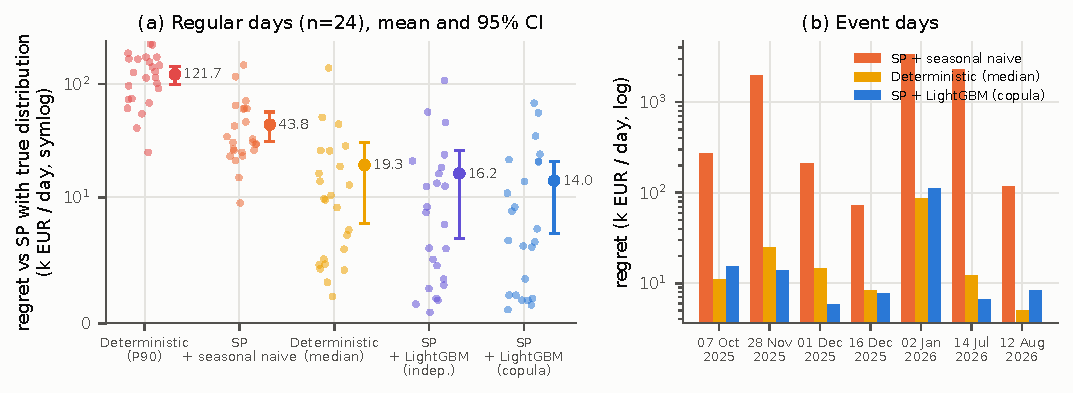
\includegraphics[width=\linewidth]{value_of_forecasts}
  \caption{(a) Daily regret on regular days (dots) with mean and 95\% confidence interval (symlog scale). (b) Event days: a forecast that does not know the retail calendar (seasonal naive) leaves millions of euros on the table on Black Friday, Prime Day and the Reyes peak.}
  \label{fig:value}
\end{figure}

\Cref{tab:value} and \cref{fig:value} support four conclusions.
\begin{enumerate}
  \item \textbf{Forecast quality dominates.} Planning with LightGBM instead of the true distribution costs \EUR{16.3}k per day on average (paired standard error \EUR{4.2}k; worse on all 31 days). This is about 0.6\% of the daily cost, or roughly \EUR{6}M per year at this volume, and it is an upper bound on what any further forecasting improvement could deliver. The seasonal-naive forecast has a regret of \EUR{44}k per day on regular days (\EUR{30}k more than LightGBM), and on event days it is catastrophic (\EUR{1.2}M per day on average): it schedules the capacity of an ordinary Friday for Black Friday.
  \item \textbf{Safety buffers are expensive.} Planning every series at its 90th percentile, a common heuristic, ignores that the 260 series do not peak together. It over-buys about 110 trucks and 50 crews per day and costs \EUR{96}k per day more than the stochastic program (paired $p<10^{-8}$), i.e.\ about \EUR{35}M per year.
  \item \textbf{The stochastic program beats the deterministic plan, modestly.} With the same LightGBM forecast, the SP with independent scenarios saves \EUR{2.9}k per day over the median plan (paired s.e.\ \EUR{1.1}k, $p=0.013$, better on 74\% of days). The SP with copula scenarios saves \EUR{3.8}k per day (s.e.\ \EUR{2.5}k, $p=0.14$). The gain is small because recourse is cheap in the base case; \cref{sec:flex} shows when it becomes large.
  \item \textbf{Correct joint calibration does not automatically pay.} The copula repairs the calibration of the national total (\cref{tab:scenarios}), but the paired cost difference to independent scenarios (\EUR{0.9}k per day) is not significant. The lesson is general: when recourse prices are nearly linear around the optimum, the plan is driven by the \emph{mean and the marginal quantiles at the critical ratio}, not by the shape of the joint distribution. Better forecasts of the level beat better forecasts of the dependence.
\end{enumerate}

